% 日本人向けのa4用紙,dvipdfmxってのとuplatexを使うよ,twocolumn--2段組だよ.
% jarticleではなく,j`s'article
% \documentclass[a4j, uplatex, dvipdfmx]{jsarticle}
\documentclass[lualatex,a4paper,ja = standard, twoside, twocolumn]{bxjsarticle}

% \documentclass の行から,\begin{document}の間をプリアンブルといいます.
% \usepackage{zemi2kai}
\usepackage{zemi2kaiLua}

% 数学関係のパッケージ
\usepackage{amsmath}
\usepackage{amsfonts}
\usepackage{ascmac}
\usepackage{theorem}
\newtheorem{defi}{定義}[section]

% 図を入れるのに使うパッケージ
% ちなみに,上の\documentclassのところにdvipdfmxと書かずに,
% \usepackage[dvipdfmx]{graphicx} って派閥があるけど,
% 個人的にはおすすめしない.
\usepackage{graphicx}

% 図を書くのに使うパッケージ
\usepackage{tikz}

% URL挿入するのに使うパッケージ
\usepackage{url}

% \newcommand{tfFrac}

\title{楽しい\LaTeX}
\author{平田研究室の誰か}
\date{\today}

\begin{document}
\maketitle
\section{文章}
  % クォーテーションマークを''hoge''とすると「左」の向きがおかしくなる
  % ``hoge''としよう!
  ``clidonci coi .i la .tamekunin. pu ciska ti''
  % 改行は1行空欄か,下のように\par をつける.原則,文章中で`\\'によって改行しない.
  \par \LaTeX は美しい文書出力を容易に実現できる software です.
  Microsoft Word (以下Word) との違いを表\ref{tbl_latexVsWord}に示しました.
    % 図や表の位置を[tbp]のように指定できる.
    % t:ページの上, b:ページの下, p: 独立したページ, h: 文中の`ここ'
    % [b]だと,ページの下に置くってこと.
    % [tbp]なら,「上,ダメなら下,それもダメなら独立したページ」
    % LaTeXの図配置は思い通りにいかない事が多い.適度な諦めも大事.
    % ちなみに,図はキャプションを下に置き,表はキャプションを上に置くので,
    % 図はページの下に,表はページの上に置くと,文字がページの中央部分にまとまるのでおしゃれ.
    \begin{table}[b]
      \center
      \caption{\LaTeX とWordの違い} \label{tbl_latexVsWord}
      \begin{tabular}{c||c|c}
        特徴 & \LaTeX & Word \\ \hline
        値段 & 無料 & 結構高い \\
        数式 & 得意 & 苦手 \\
        Linuxで & 動く & 動かない \\
        出力品質 & 高い & 低い \\
        自由か? & 自由 & proprietary \\
        source control & Git等で容易 & 困難 \\
        WYSIWYGか? & じゃない & そう \\
        春名先生が & 嫌い & 嫌いじゃない \\
        爲國が & 好き & 好きじゃない
      \end{tabular}
    \end{table}
  そんな\LaTeX は
    \begin{itemize}
      \item 卒論・修論・博論
      \item 論文
      \item 進捗資料
      \item 授業レポート
      \item 就職活動における添え状
      \item 履歴書
      \item 恋文
      \item 始末書
      \item 退職届
      \item 遺言
    \end{itemize}
  等々の人生のあらゆる場面で必要となる文書を作成する際に役立つでしょう.

\section{数式}
  文章には数式がつきもの$^\text{[要出典]}$,
  前述のように,\LaTeX で文章を作成するメリットは数式を容易に挿入可能である.
  例えば,文中で,
  $\operatorname{card}(\mathbb{R}) = \operatorname{card}(\mathbb{R}^2)$のように.
  % 以後では「線型代数の初歩」をテーマに文章を書きました.
  % \subsection{固有値}
  %     \begin{defi}[固有値]
  %       行列$A$に対して,
  %         \[
  %           Av = \lambda v
  %         \]
  %       を満たす0でないベクトル$v$\footnote{
  %           「え,ベクトルって太字か二重文字で書くんじゃないの?」と思うかもしれませんが,
  %           分野によっては「みりゃあわかるでしょwww」ということで普通の文字で書きます.
  %         }を「固有ベクトル」,$\lambda$を「固有値」という.
  %     \end{defi}
  %   行列にベクトルを作用させると,通常は「向き」が変わります.例えば,
  %     \begin{equation}
  %       \begin{bmatrix}
  %         4 & 12 \\
  %         6 & 14
  %       \end{bmatrix}
  %       \begin{bmatrix}
  %         1 \\ 2
  %       \end{bmatrix} =
  %         \begin{bmatrix}
  %           2 \\ 16
  %         \end{bmatrix}
  %     \end{equation}
  %   ですが,行列を掛ける前のベクトル$[1, 2]^\top$をいくら伸ばしたり縮めても,
  %   行列を掛けたあとの行列$[2, 16]^\top$にはなりません.
  %   これは行列を掛けたことによって向きが変わったと解釈できます.
  %   しかし,あるベクトルは向きが変わらず長さのみが変化します.例えば,
  %     \begin{equation}
  %       \begin{bmatrix}
  %         4 & 12 \\
  %         6 & 14
  %       \end{bmatrix}
  %       \begin{bmatrix}
  %         1 \\ -1
  %       \end{bmatrix} =
  %         \begin{bmatrix}
  %           8 \\ -8
  %         \end{bmatrix} = 8
  %           \begin{bmatrix}
  %             1 \\ -1
  %           \end{bmatrix}
  %     \end{equation}
  %   となります.行列を掛ける前のベクトルを8倍すれば,行列を掛けたあとのベクトルと同じ,
  %   つまり行列を掛けても向きが変わらないということです.
  %   まとめると,
  %     \begin{itemize}
  %       \item 固有ベクトル\\
  %         ある行列に対して,行列を掛けても向きが変わらないベクトル.
  %       \item 固有値\\
  %         固有ベクトルに行列を掛けたとき,どのくらい伸び縮みするかの倍数.
  %     \end{itemize}
  %   となります.
  %   \subsubsection{固有値と固有ベクトルの求め方}
  %     固有ベクトルを求める前に,固有値を求めます.
  %     固有値と固有ベクトルの定義から,
  %       \begin{align}
  %         Av &= \lambda v \\
  %         Av - \lambda v &= 0 \\
  %         \left(A - \lambda \mathrm{E} \right)v &= 0 \label{eq_eig}
  %       \end{align}
  %     となります.ここで,もし,$A - \lambda \mathrm{E}$に逆行列が存在すると,
  %     $\left(A - \lambda \mathrm{E} \right)^{-1}$を左からかけて,$v = 0$となってしまいます.
  %     ということは,$A - \lambda \mathrm{E}$に逆行列が存在しなければ好都合です.
  %     つまり,
  %       \begin{equation}
  %         \operatorname{det}\left(A - \lambda \mathrm{E} \right) = 0
  %       \end{equation}
  %     となれば良いということです.固有値を求めたあと,求めた固有値に対して固有ベクトルが求まります.
  \par ゴッツイ式は別立てして書くのが普通.式番号がいらない場合は,
    \[
      \forall \epsilon > 0 \quad \exists \delta > 0 \quad
      \text{s.t.} \quad
        \|x(0)\| < \delta \Rightarrow ||x(t)|| < \epsilon
    \]
  式番号がいる場合は,
    \begin{equation}
      \operatorname{dim}\operatorname{Ker}
        \exp(A) \neq 0
    \end{equation}
  みたいな感じ.ここで気をつけてほしいのは,
  $\sin$とか$\exp$みたいな「みんなが知ってる関数」を
  $sin$, $exp$みたいにイタリック\footnote{斜めになってる字のこと.
    ただし,イタリックのことを「斜体」というと組版警察やフォント警察に叩かれる.}で書くとクソダサい.
  \par 括弧の中の式が`大きい'場合は,一工夫しないと左みたいに見苦しくなる.
    \begin{equation}
      57(\frac{1}{s^2 + 2s + 1} + 2) =57\left(\frac{1}{(s + 1)^2} + 2 \right)
    \end{equation}
  複数の式が続く場合,\texttt{align}環境を使う.
  \texttt{eqnarray}環境だとスペースの両端の空白が大きくてダサい.
    % 揃えたい記号の直前に&を置く
    \begin{align}
      \sin(x) &= \sin(x + 2\pi) \\
      &= \sum_{n = 0}^{\infty} (-1)^{n}\frac{x^{(2n + 1)}}{(2n + 1)!}
    \end{align}
\section{図}
  しばしば図を入れる機会がある,例えば,図\ref{pht_doyle}みたいに.
    % 図番号を自分で考えて書く必要はない.
    % \caption{hoge}の横に\label{fuga}と書いておけば,
    % 文中で\ref{fuga}とする図番号を適当に入れてくれる.
    \begin{figure}[tbp]
      % \begin{center} ~ \end{center}とすると,
      % 図の周りの余白が大きくなってしまう.
      % \centeringがおすすめ.何より1行で済む.
      \centering
      % width = 0.95\columnwidth ← 文の横幅の0.95倍を図の横幅にする
      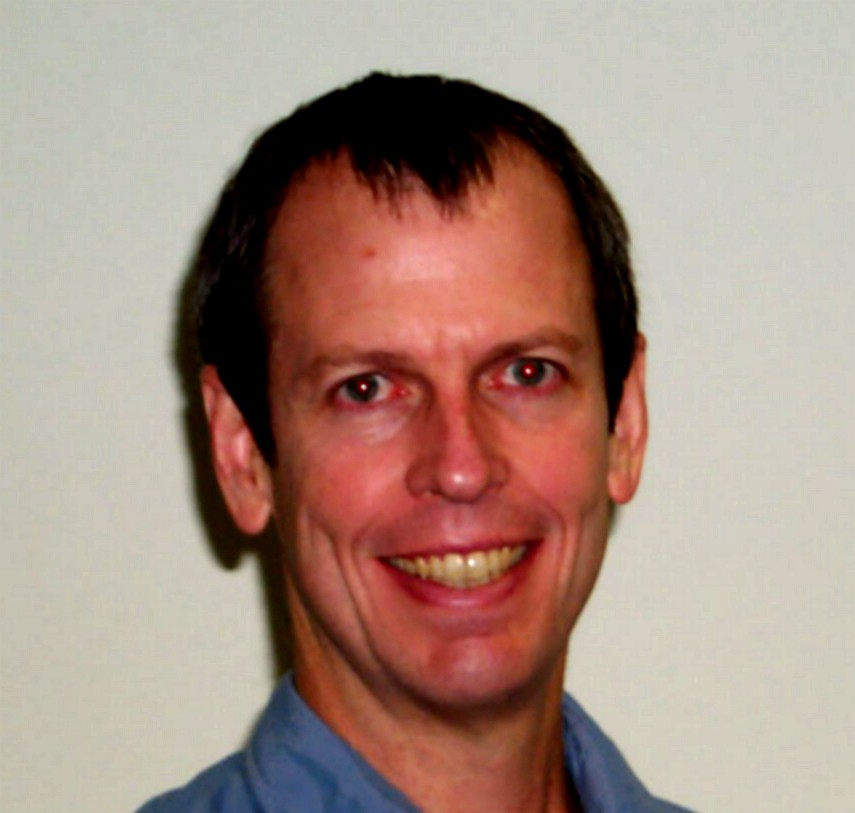
\includegraphics[width = 0.95\columnwidth]{figure/doyle_photo.jpg}
      \caption{すごい人} \label{pht_doyle}
    \end{figure}
  \subsection{ラスター画像とベクター画像}
    原則として,進捗資料に掲載する図はベクター画像です.
    図\ref{fig_ciclesonide}はベクター画像で,いくら拡大してもドットが見えません.
      \begin{figure}[tbp]
        \centering
        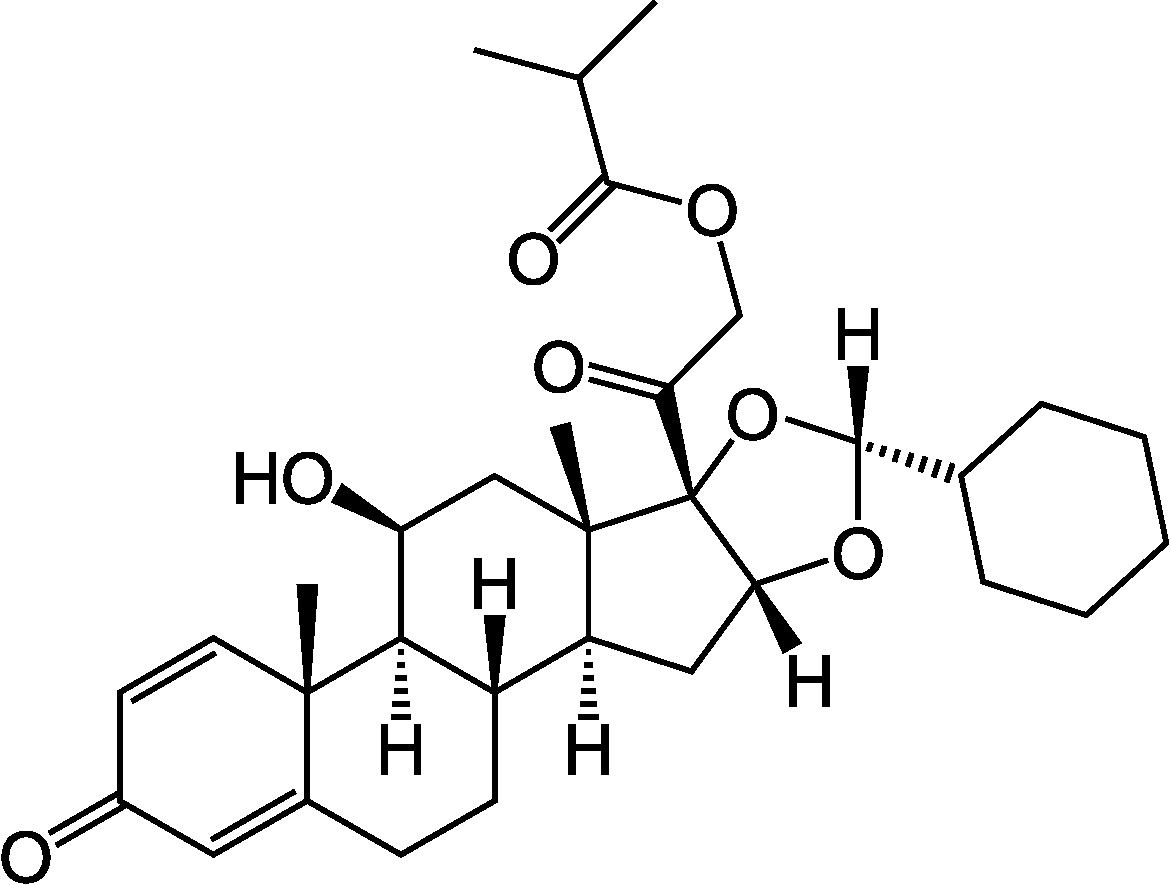
\includegraphics[width = 5cm]{figure/chemi_vec.pdf}
        \caption{ベクター画像の例: いくら拡大しても粗が目立たない.} \label{fig_ciclesonide}
      \end{figure}
    通常のデジカメで撮影した写真や,出典元がラスター画像しか用意していない場合には,
    図\ref{pht_doyle}のようにラスター画像を使ってください.
\section{楽しいLua\LaTeX}
  将来,こんなことが起きるかもしれません.
    \begin{screen}
      3歳娘「パパ (ママ),文中に入れた伝達関数が安定か判定するマクロを作って.」\\
      3歳娘「Matlab, Scilabを行き来せずに,.texファイルの編集が即反映されるようにして.」\\
      3歳娘「みんな持ってるの」\\
      3歳娘「私だけ持ってないの」\\
      ワイ「(どうやって,実装したらええんや……)」
    \end{screen}
  \TeX 言語だけで,伝達関数の安定性を判別するのは難しいかもしれません.
  しかし,Lua\LaTeX を使えば,簡単に実行できます.


\section{その他}
  \url{https://ichiro-maruta.blogspot.com/2013/03/latex.html} \\
  \url{https://www.math.tohoku.ac.jp/tmj/oda_tex.pdf}\\
  この辺読んどいて.ネットでググった情報や,先輩からもらったファイルは糞古い書き方とか,
  正しくない書き方とかが残されているので全部うのみにするのはアレ.

\end{document}
